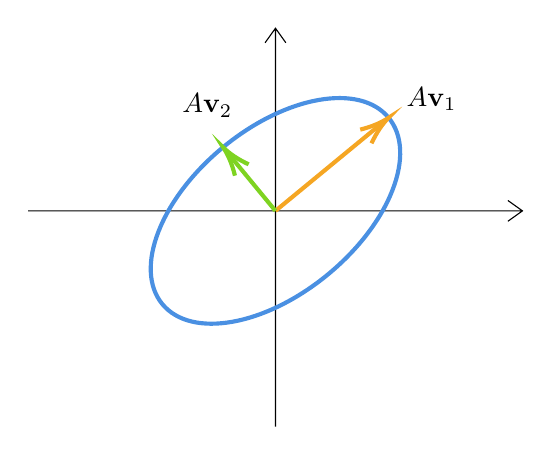
\begin{tikzpicture}[x=0.75pt,y=0.75pt,yscale=-1,xscale=1]
%uncomment if require: \path (0,300); %set diagram left start at 0, and has height of 300

%Shape: Axis 2D [id:dp5842664307886825] 
\draw  (216,137) -- (454.11,137)(335.11,49) -- (335.11,241) (447.11,132) -- (454.11,137) -- (447.11,142) (330.11,56) -- (335.11,49) -- (340.11,56)  ;
%Shape: Ellipse [id:dp9660000625734635] 
\draw  [color={rgb, 255:red, 74; green, 144; blue, 226 }  ,draw opacity=1 ][line width=1.5]  (280.59,181.88) .. controls (266.65,164.95) and (279.76,131.13) .. (309.87,106.34) .. controls (339.99,81.55) and (375.7,75.18) .. (389.64,92.12) .. controls (403.58,109.05) and (390.46,142.87) .. (360.35,167.66) .. controls (330.24,192.45) and (294.52,198.82) .. (280.59,181.88) -- cycle ;
%Straight Lines [id:da36332977734700256] 
\draw [color={rgb, 255:red, 245; green, 166; blue, 35 }  ,draw opacity=1 ][line width=1.5]    (335.11,137) -- (387.32,94.02) ;
\draw [shift={(389.64,92.12)}, rotate = 140.54] [color={rgb, 255:red, 245; green, 166; blue, 35 }  ,draw opacity=1 ][line width=1.5]    (14.21,-4.28) .. controls (9.04,-1.82) and (4.3,-0.39) .. (0,0) .. controls (4.3,0.39) and (9.04,1.82) .. (14.21,4.28)   ;
%Straight Lines [id:da7831499075107744] 
\draw [color={rgb, 255:red, 126; green, 211; blue, 33 }  ,draw opacity=1 ][line width=1.5]    (335.11,137) -- (311.78,108.65) ;
\draw [shift={(309.87,106.34)}, rotate = 50.54] [color={rgb, 255:red, 126; green, 211; blue, 33 }  ,draw opacity=1 ][line width=1.5]    (14.21,-4.28) .. controls (9.04,-1.82) and (4.3,-0.39) .. (0,0) .. controls (4.3,0.39) and (9.04,1.82) .. (14.21,4.28)   ;

% Text Node
\draw (397,76.4) node [anchor=north west][inner sep=0.75pt]    {$A\mathbf{v}_{1}$};
% Text Node
\draw (289,79.4) node [anchor=north west][inner sep=0.75pt]    {$A\mathbf{v}_{2}$};


\end{tikzpicture}